\documentclass[conference]{../IEEEtran}

\usepackage{graphicx}
\usepackage{amsmath}
\usepackage{amssymb}
\usepackage{algorithm}
\usepackage{subfigure}
\usepackage{algpseudocode}
\usepackage{multirow}
\usepackage{pdfsync}
\usepackage{siunitx}
\usepackage{url}
\usepackage{array,graphicx}

\providecommand{\e}[1]{\ensuremath{\times 10^{#1}}}

\begin{document}

\title{Lab 4: Particle Filter}
\author{Olivier Cheng, Yukun Lin and Jennifer Zheng}
\bstctlcite{IEEEexample:BSTcontrol}
\maketitle

\begin{abstract}
A key ability for a mobile robot is its ability to localize itself in a known environment.
In this paper, a particle filter is presented that can localize a Jaguar Lite Vehicle in a known start position using odometry and laser range scanner measurements.
In simulation, the maximum position error was \SI{0.05}{\meter} over a \SI{300}{\second} test.
In hardware, the particle filter's estimate of the trajectory performed better than odometry alone, but the accuracy of the state estimate cannot be determined without a method of tracking the robot's true position.
In addition, implementing the Augmented Monte Carlo Localization (MCL) algorithm can solve the unknown start position and kidnapped robot problem in a non-symmetric map.
Future work in localization includes adding features to symmetric maps, increasing the number of particles, and tuning the MCL constants.

\end{abstract}


%%%%%%%%%%%%%%%%%%%%%%%%%%%%%%%%%%%%%%%%%%%%%%%%%%%%%%%%%%%%%%%%%%%%%%%%%%%
\section{Introduction}
%%%%%%%%%%%%%%%%%%%%%%%%%%%%%%%%%%%%%%%%%%%%%%%%%%%%%%%%%%%%%%%%%%%%%%%%%%%
To make good decisions in a known environment, an autonomous mobile robot such as the
Jaguar Lite must to be able to accurately determine its pose using onboard sensors.
However, the localization problem is challenging for several reasons; sensor readings can
be noisy, and symmetries in the environment makes it impossible create a bijection from
the set of sensor readings to the set of robot poses.

To address these challenges, a particles filter localization was implemented in this lab
to determine the 2D position and orientation of the Jaguar Lite robot in a known
environment. Odometry measurements were used to predict the position and orientation of
the robot, and measurements from the laser scans were then used to correct this
prediction. It is shown in this report that the implemented particle filter is able to
localize the robot starting from both known and unknown position.

%%%%%%%%%%%%%%%%%%%%%%%%%%%%%%%%%%%%%%%%%%%%%%%%%%%%%%%%%%%%%%%%%%%%%%%%%%%
\section{Background}
%%%%%%%%%%%%%%%%%%%%%%%%%%%%%%%%%%%%%%%%%%%%%%%%%%%%%%%%%%%%%%%%%%%%%%%%%%%
The Jaguar is a track driven robot developed by Dr. Robot Inc. It can operate on rough
terrains and is equipped with outdoor GPS, a 6-DOF IMU, encoders, a high-resolution video
camera, and a laser scanner.  The laser scanner has a maximum range of \SI{5.6}{\meter}
and scanning angle of \SI{240}{\degree} with a resolution of \SI{0.25}{\degree}.

While the odometry with the wheel encoders can be used to estimate the position and
orientation of the robot through dead-reckoning given a known starting position, a build
up of random errors from odometry will lead to an unbounded growth of localization error
as the robot travels further.  It is therefore necessary to integrate measurements from
the laser scanner to bound this error.

%%%%%%%%%%%%%%%%%%%%%%%%%%%%%%%%%%%%%%%%%%%%%%%%%%%%%%%%%%%%%%%%%%%%%%%%%%%
\section{Particle Filter}
%%%%%%%%%%%%%%%%%%%%%%%%%%%%%%%%%%%%%%%%%%%%%%%%%%%%%%%%%%%%%%%%%%%%%%%%%%%
A particle filter was used to combine encoder and laser range scanner measurements for
robot localization. In a particle filter, a set of particles is used, to represent a
belief state of the robot's position and heading. Each particle represents a single
``guess'' of the robot's pose, and has a weight that indicates the likelihood of the robot
being in that pose.

%%%%%%%%%%%%%%%%%%%%%%%%%%%%%%%%%%%%%%%%%%%%%%%%%%%%%%%%%%%%%%%%%%%%%%%%%%%
\subsection{Initialization}
%%%%%%%%%%%%%%%%%%%%%%%%%%%%%%%%%%%%%%%%%%%%%%%%%%%%%%%%%%%%%%%%%%%%%%%%%%%

Each particle $p$ is the vector $[x\; y\; \theta]$ which represents the planar position
$(x,y)$ and heading $\theta$ of the particle. In the initialization step of the particle
filter, a set of particles is generated randomly, where $x$, $y$, and $\theta$ are drawn
from continuous uniform distributions.  The bounds of the uniform distributions depends on
the confidence in the starting state of the  robot; smaller bounds are used when there is
high confidence, and larger bounds are used when there is low confidence.

%%%%%%%%%%%%%%%%%%%%%%%%%%%%%%%%%%%%%%%%%
\subsection{Prediction Step}
%%%%%%%%%%%%%%%%%%%%%%%%%%%%%%%%%%%%%%%%%

In the prediction step, each particle's position and orientation is updated using
odometry. Encoder measurements are used to calculate the robot's displacement $\Delta v$
and change in orientation $\Delta \theta$. For each particle, it's position and heading is
updated using $\Delta v + \epsilon_v$ and $\Delta \theta + \epsilon_{\theta}$, where
$\epsilon_v$ and $\epsilon_{\theta}$ are noise drawn from a normal distribution centered
at zero.


%%%%%%%%%%%%%%%%%%%%%%%%%%%%%%%%%%%%%%%%%
\subsection{Correction Step}
%%%%%%%%%%%%%%%%%%%%%%%%%%%%%%%%%%%%%%%%%

The measurements of beams from the laser scanners $\vec{z}$ are used to assign a weight to
each particle. The assigned weight is based on the difference between  the expected
measurement $\vec{z}_{exp}$ given a particle's state and $\vec{z}$.

To calculate $\vec{z}_{exp}$, it is necessary to find the closest wall that a laser beam
will reflect off given a particle's position and heading, and the distance that the laser
beam has traveled to hit that wall.

\subsubsection{Closest Wall Distance}

Let a wall segment with endpoints $(x_1$, $y_1)$ and $(x_2$, $y_2)$ in the global frame
with length $\alpha$ be described by the parametric equation
\begin{equation}
  W(t_w) = \begin{bmatrix}
    x_1\\y_1
    \end{bmatrix} +
    \begin{bmatrix}
    x_m\\ y_m
  \end{bmatrix} t_w
  \label{eq:wallSeg}
\end{equation}
where
\begin{equation}
  x_m = \frac{x_2-x_1}{\alpha} \quad \text{and} \quad y_m = \frac{y_2-y_1}{\alpha}
\label{eq:unit}
\end{equation}
Observe that Eq.~\ref{eq:wallSeg} describes all points on the wall if and only if $t_w \ge
0$ and $t_w < \alpha$.

Let the robot be at position $(x,y)$ with a beam from its laser scanner emitting at a
heading of $\theta$ in the global frame.  The ray of this laser beam can be described by
the parametric equation
\begin{equation}
  L(t_l) =
  \begin{bmatrix}
    x\\y
    \end{bmatrix} +
    \begin{bmatrix}
    \cos \theta\\
    \sin \theta
  \end{bmatrix} t_l
  \label{eq:laser}
\end{equation}
Observe that setting Eq.~\ref{eq:tl} to Eq.~\ref{eq:tw} gives the intersection point of
the two lines described by Eq.~\ref{eq:tl} and Eq.~\ref{eq:tw}. It can be shown that
\begin{equation}
  t_l = \frac{x_m(y-y_1)+y_m(x_1-x)}{y_m\cos\theta - x_m\sin\theta}
  \label{eq:tl}
\end{equation}
and
\begin{equation}
  t_w = \frac{(y-y_1)\cos\theta + (x_1-x)\sin\theta}{y_m\cos\theta-x_m\sin\theta}
\label{eq:tw}
\end{equation}
satisfies the condition of $W(t_w) = L(t_l)$.

It follows that the intersection point will be a point on the wall segment from the laser
beam traveling away from the robot if and only if $t_w, t_l > 0$ and and $t_l < \alpha$.
Given that these conditions are true, then the Euclidean distance of $[x\;y]$ and $L(t_l)$
will give the distance traveled by the laser beam to the wall segment defined by
Eq.~\ref{eq:wallSeg}.

For a map with multiple wall segments, the distance traveled by the laser beam to each
wall segment is first calculated, and the wall segment that corresponds to the least
distance traveled by the laser beam is used.

\subsubsection{Weight Calculation}

For each particle, $\vec{z}_{exp}$ is calculated by iterating through the available beams
of the laser scanners in steps of 5 and calculating the expected closest wall distance for
each beam of interest. Note that in the case that a laser beam does not intersect with a
wall segment, the max laser range of \SI{5.6}{\meter} is used instead.

The difference between the expected and actual measurement is given by
\begin{equation}
  \vec{\epsilon} = \vec{z}_{exp} - \vec{z}.
\end{equation}
Each element in $\vec{\epsilon}$ is given a weight using the probability distribution
function of a Gaussian centered at zero with variance $\sigma^2_w$ with some added minimum
weight. The weight of a particle $p_i$ is therefore given by $w_i = \prod \vec{\epsilon}$.

\begin{figure}[t]
  \centering
  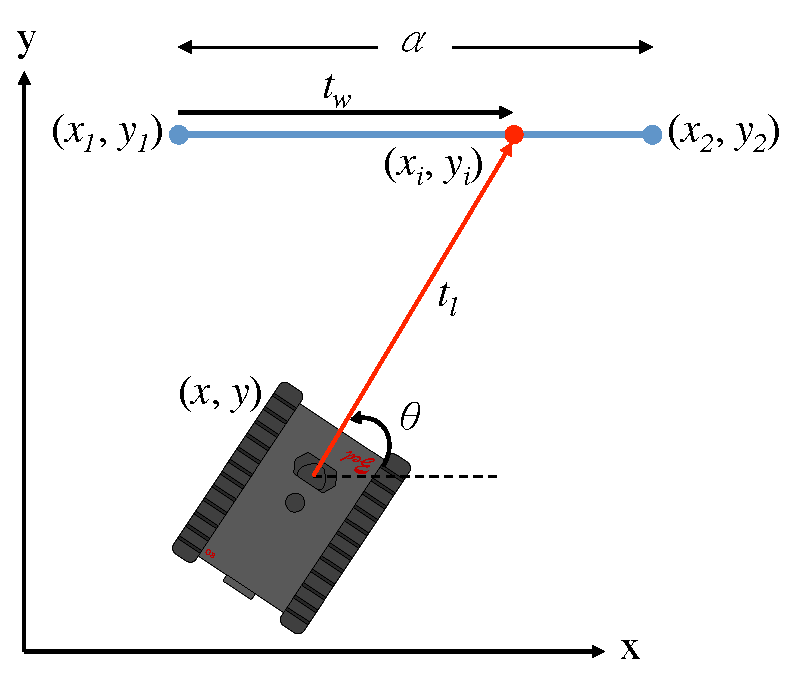
\includegraphics[width=2.5in]{figures/Untitled.pdf}
  \label{fig:wallSeg}
  \caption{Labeled graph of the robot at position ($x,y$) and a laser
           scan to the wall.}
\end{figure}

\subsubsection{Importance Sampling}

The particles are then re-sampled with replacement, to create a new set of particles. The
probability of a particle $p_i$ being chosen is directly proportion to its weight $w_i$. A
low variance re-sampler from \textit{Probabilistic Robotics} was implemented because it is
exact and has a run time linear to the number of particles.


\begin{figure*}[t]
  \centering
  \subfigure[]{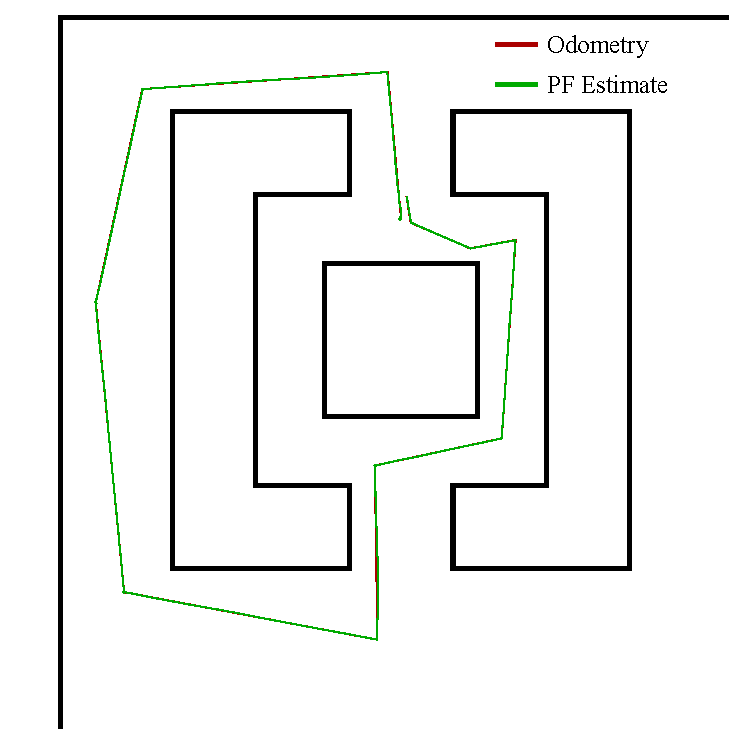
\includegraphics[width = 6cm]{figures/sim_traj.pdf}
  \label{fig:simSpread}}
  \hspace{.5 cm}
  \subfigure[]{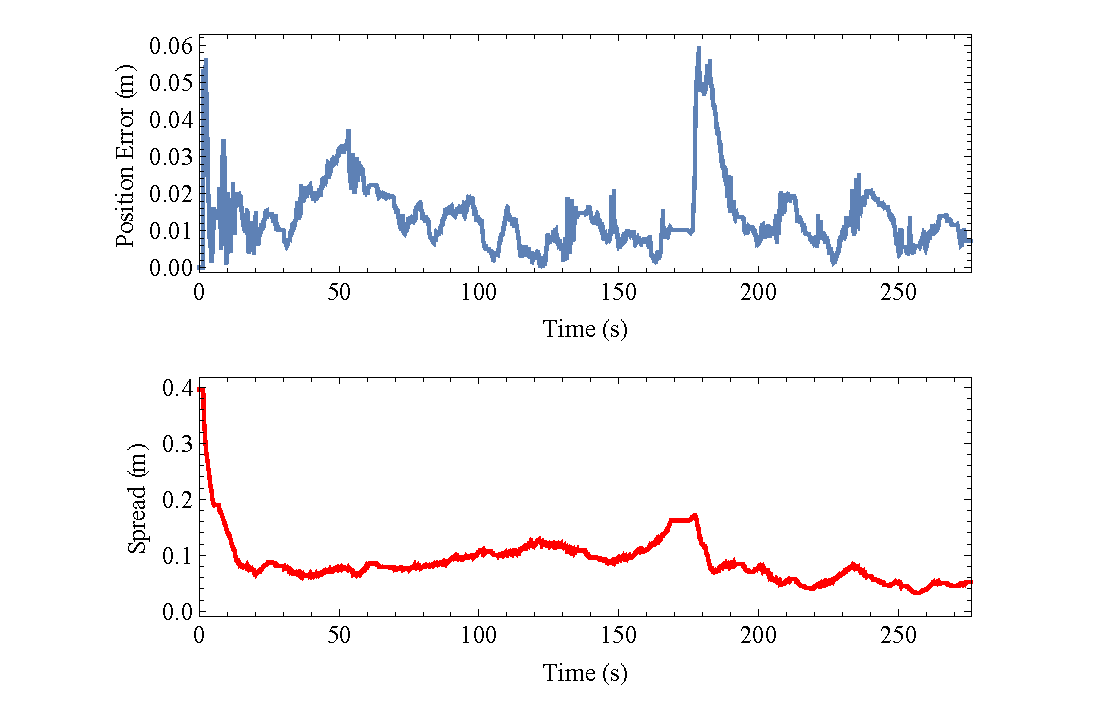
\includegraphics[width = 10cm]{figures/sim_known_start.pdf}
  \label{fig:simKnown}}
  \caption{Fig.~\ref{fig:simSpread} shows the trajectory plot of the Jaguar as tracked by
           odometry (red) and the particle filter (green). Fig.~\ref{fig:simKnown} shows both the
           difference between the odometry and particle filter estimates and the standard deviation
           of the particles. These plots refer to the simulation test for a known start position.}
\end{figure*}

%%%%%%%%%%%%%%%%%%%%%%%%%%%%%%%%%%%%%%%%%
\subsection{Kidnapped Robot and Unknown Start Position}
%%%%%%%%%%%%%%%%%%%%%%%%%%%%%%%%%%%%%%%%%

In this lab, we have assimilated the lost robot case to the unknown start position. When
the initial position of the robot is not known, the initial set of particles are spread
across a wide area of the map.  Due to symmetries in the map (such as long corridors), it
is possible for the particles to converge to  the wrong location. This leads to a
situation called particle deprivation, when none of the particles are in the vicinity of
the location of the actual robot. Particle deprivation can also happen in the case the
kidnapped robot when it is carried to an arbitrary location.

Particle deprivation can be accounted for by adding random particles during the correction
step instead of re-sampling. The augmented MCL algorithm described in
\textit{Probabilistic Robotics} is used for that purpose in this lab. Augmented MCL works
by keeping track of the long term and short term average weight of the particles denoted
by $\omega_{slow}$ and $\omega_{fast}$ respectively.

In each iteration of the particle filter, $\omega_{slow}$ and $\omega_{fast}$ are updated
based on the average particle weights $\omega_{avg}$ based on the equations
\begin{equation}
  \omega_{slow} = \omega_{slow} + \alpha_{slow} * (\omega_{avg} + \omega_{slow})
  \label{eq:sh_term}
\end{equation}
and
\begin{equation}
  \omega_{fast} = \omega_{fast} + \alpha_{fast} * (\omega_{avg} + \omega_{fast})
  \label{eq:lo_term},
\end{equation}
where the constants $\alpha_{slow} < \alpha_{fast}$ and $0 < \alpha_{slow},
\alpha_{fast} < 1$. During the correction step, there is a probability of
\begin{equation}
  \rho = \text{max}(0, 1- \omega_{fast} / \omega_{slow})
  \label{eq:rho}
\end{equation}
of re-sampling a particle based of weights versus adding a new particle with a random
state.

This means that in the cases of particle deprivation, a sharp drop in $\omega_{avg}$ will
drive $\rho$ to zero according to Eq.~\ref{eq:rho}, due to $\omega_{fast}$ decreasing
faster than $\omega_{slow}$, causing new random particles to be added in the next few
iterations of the correction step. But as $\omega_{slow}$ starts decreasing as well,
$\rho$ will start increasing again, giving the newly introduced particles to converge to
the right location.

%%%%%%%%%%%%%%%%%%%%%%%%%%%%%%%%%%%%%%%%%%%%%%%%%%%%%%%%%%%%%%%%%%%%%%%%%%%
\section{Results and Discussions}
%%%%%%%%%%%%%%%%%%%%%%%%%%%%%%%%%%%%%%%%%%%%%%%%%%%%%%%%%%%%%%%%%%%%%%%%%%%
The particle filter was tested in both simulation and hardware.  Experiments were done for
both cases of known start position and unknown start position. In simulation, the true
trajectory of the robot was tracked based on the simulated odometry measurements.
Position error is defined as
\begin{equation}
  \epsilon = \sqrt{(x_o-x_{pf})^2+(y_o-y_{pf})^2}
\end{equation}
where the odometry position is given by $(x_o,y_o)$ and the particle filter estimate of
the position is given by $(x_{pf},y_{pf})$. The spread of the particles is defined by
\begin{equation}
  s = \sqrt{\sigma_x^2+\sigma_y^2}
\end{equation}
where $\sigma_x$ and $\sigma_y$ are the standard deviations of the particles in the $x$
direction and $y$ direction respectively.

%%%%%%%%%%%%%%%%%%%%%%%%%%%%%%%%%%%%%%%%%
\subsection{Simulation: Known Start Position}
%%%%%%%%%%%%%%%%%%%%%%%%%%%%%%%%%%%%%%%%%

Since the robot starts at a known position, the particles are spread in a 4 by
\SI{4}{\meter} square centered around the robot's start position. The particles converge
towards the actual position of the simulated robot after less than \SI{1}{\second}
(Fig.~\ref{fig:simKnown}.  Therefore, the state estimate is able to track the odometry
with a maximum position error of about \SI{5}{\meter} (Fig.~\ref{fig:simKnown}).  In
Fig.~\ref{fig:simKnown}, there is a spike in the position error around \SI{175}{\second},
which may be caused by the random noise added to the odometry.  Fig.~\ref{fig:simKnown},
shows that, after the initial prediction and correction step, the spread stays under
\SI{0.2}{\meter}.  Visual observations of Fig.~\ref{fig:simSpread} show the particle
filter estimate overlaying the odometry trajectory, demonstrating that the particle filter
can be used as a localization method for a known start position.

\begin{figure*}[t]
  \centering
  \subfigure[]{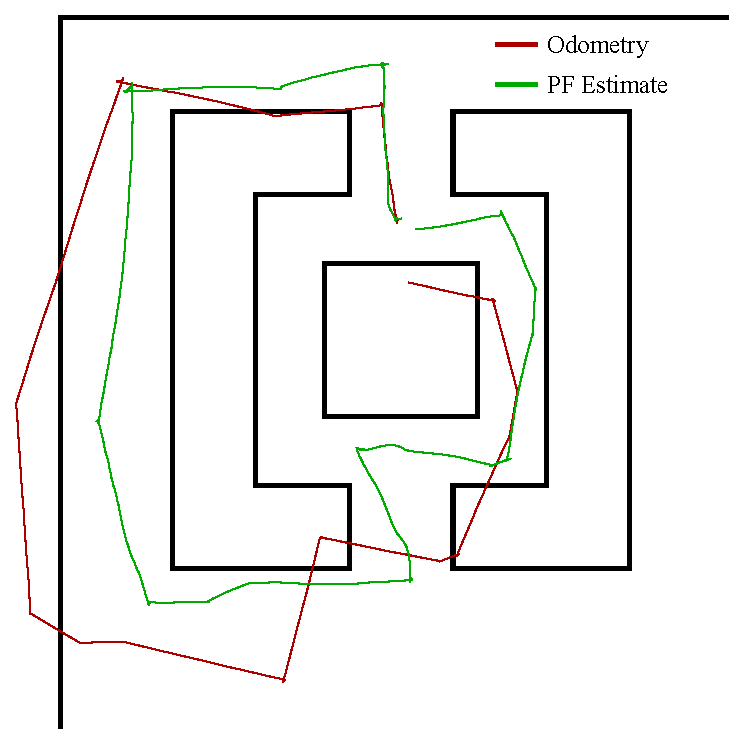
\includegraphics[width = 6cm]{figures/hardware_traj.pdf}
  \label{fig:hardTraj}}
  \hspace{.5 cm}
  \subfigure[]{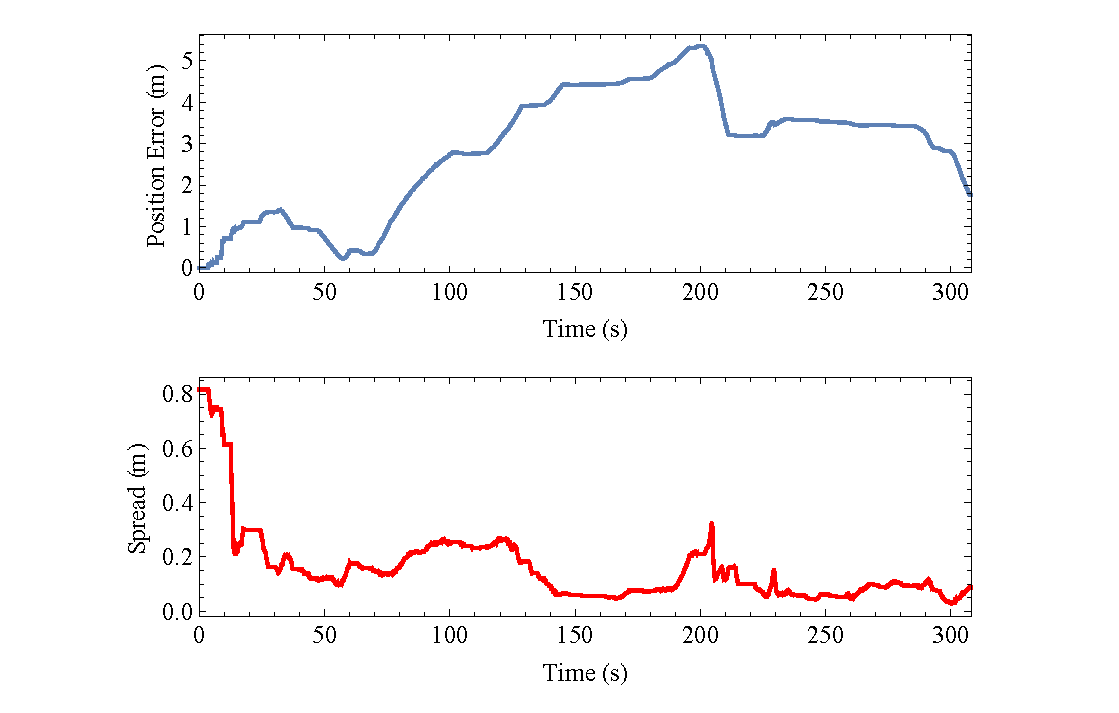
\includegraphics[width = 10cm]{figures/hardware_large_spread.pdf}
  \label{fig:hardSpread}}
  \caption{Fig.~\ref{fig:hardTraj} shows the trajectory
  plot of the Jaguar as tracked by odometry (red) and the
  particle filter (green). Fig.~\ref{fig:hardSpread} shows
  both the difference between the odometry and particle
  filter estimates and the standard deviation of the particles.}
  \label{fig:hardware}
\end{figure*}


\begin{figure}[t]
\centering
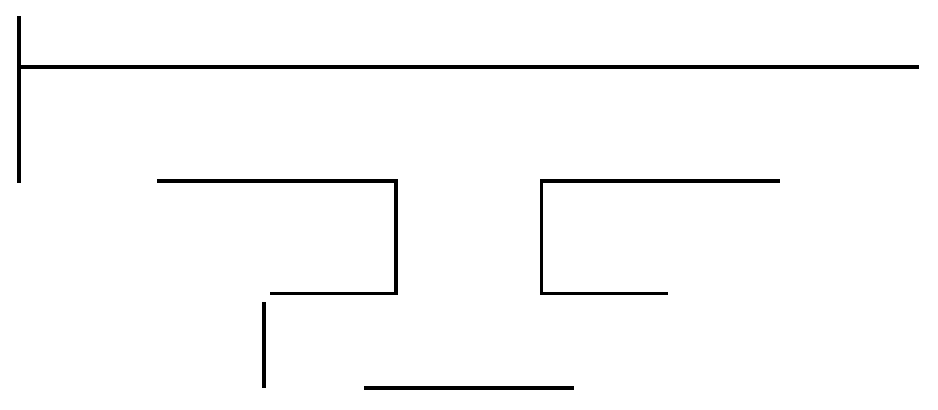
\includegraphics[width=2.5in]{figures/small_map.pdf}
\label{fig:usmap}
\caption{Unsymetric map on x axis}
\end{figure}


%%%%%%%%%%%%%%%%%%%%%%%%%%%%%%%%%%%%%%%%%
\subsection{Simulation: Unknown Start Position}
%%%%%%%%%%%%%%%%%%%%%%%%%%%%%%%%%%%%%%%%%

With an unknown start position case in simulation, the map was modified to be asymmetrical
in its principal component axis as shown in Fig.~\ref{fig:usmap}. This was done to speed
up convergence by decreasing the chances that the particles converged to an incorrect
symmetrical position.

The particles spread generally decrease in total over time when the robot moves around
meaning that the particles are converging towards the state that has the most likelihood
to be the position of the robot.  The spread of the particles can sometimes suddenly
increase sharply and that can happen, for instance, when the robot's laser scanner is
reaching a corner that has similarity with another corner on the map.

%%%%%%%%%%%%%%%%%%%%%%%%%%%%%%%%%%%%%%%%%
\subsection{Hardware: Known Start Position}
%%%%%%%%%%%%%%%%%%%%%%%%%%%%%%%%%%%%%%%%%
Using the Jaguar, the particle filter was tested around the flower beds outside of Parsons
Engineering Building.  Fig.~\ref{fig:hardTraj} shows the Jaguar's odometry measurements
and particle filter state estimates relative to the flower beds.  Based solely on the
odometry data, the Jaguar's trajectory travels through the wall and flower bed.  This
error may come from slipping and illustrates the need for a correction step in
localization.  The localization with the particle filter gives realistic position
estimates.  However, the accuracy of this method cannot be quantified without the actual
Jaguar trajectory.

The spread of the particles is shown in Fig.~\ref{fig:hardSpread}. There are two
interesting regions in the spread.  From $t=75$ to $t=150$ the spread increases to
\SI{0.3}{\meter}.  This occurs along the long corridor on the left side of the map in
Fig.~\ref{fig:hardTraj}.  The particles spread along the Jaguar's $x$-axis because of the
lack of defining features.  For example, if a particle was one meter behind the Jaguar
along that corridor, the predicted laser scans would match the measured scans.  Thus, the
spread widens because particles farther from the state estimate are given similar weights
to particles actually estimating the Jaguar's position.

This is a limitation of the particle filter implemented.  In areas with symmetry and
lacking defining feature, the spread can increase, indicating uncertainty in the filter's
estimate.  Possible methods of overcoming this limitation include adding obstacles or
defining features, improving the odometry measurements to reduce the random noise in the
prediction step, or increasing the number of particles.

From $t=190$ to $t=220$, the spread increases again.  This occurs when the Jaguar is
entering back into the small square from the bottom of the map in Fig.~\ref{fig:hardTraj}.
The spread may come from residual spread in the $x$-axis of the Jaguar after leaving the
long corridor.  In addition, the bottom of the map has empty space where the Jaguar's
laser scans reach their max range.  This makes it difficult for the particle filter to
localize for similar reasons to the long corridor.  There are multiple positions that can
provide the same laser scan readings.


\begin{figure}[t]
  \centering
  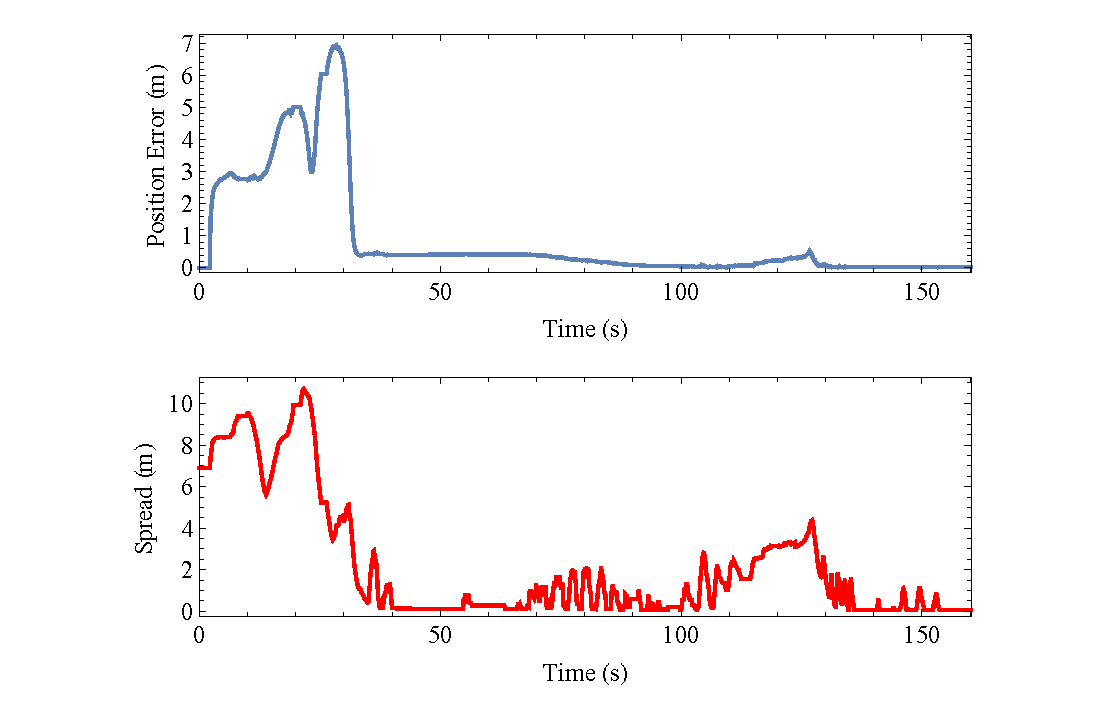
\includegraphics[width=9cm]{figures/sim_unknown_start_error.pdf}
  \label{fig:sim_unknown_err}
  \caption{Position error and spread in simulation with an unknown start position}
\end{figure}

%%%%%%%%%%%%%%%%%%%%%%%%%%%%%%%%%%%%%%%%%
\subsection{Hardware: Unknown Start Position}
%%%%%%%%%%%%%%%%%%%%%%%%%%%%%%%%%%%%%%%%%
The particle filter was tested on the Jaguar with an unknown start position.  The
performance of the filter had inconsistent convergence times likely due to several
factors.  The Jaguar was tested using the same symmetric as for known start position.
While the map is only symmetric across the $y$-axis, there are local symmetries that the
particles can cluster around.  Thus, based on where the particles are randomly
distributed, the particles can converge quickly if they are distributed around the robot's
position, or it can converge slowly if they are distributed around a local symmetry.

Adding more particles may also improve the particle performance.  For the unknown start
position, the particle filter was run with 1000 particles.  However, the greater the
number of particles, the increased likelihood that the particle will be distributed near
the robot.  A limitation of increasing the number of particles is run time of the code.
Each particle goes through the correction step, which calculates the particle's distance
from each wall.  This can be costly depending on how often the control loop is run, how
many laser scans are being used, and how large the map is since the calculating the
distance to the wall uses the square root function.

In addition, the heading of the particles can influence the convergence.  The particle
filter implemented creates randomly distributed particles with random headings.  So, even
if a particle lands near the Jaguar but has a different heading, it will be resampled.
One way to correct for this is to take each particle, check the estimated laser scans for
multiple headings, and choose the heading with the higher weight.

\addtolength{\textheight}{-20cm}


%%%%%%%%%%%%%%%%%%%%%%%%%%%%%%%%%%%%%%%%%%%%%%%%%%%%%%%%%%%%%%%%%%%%%%%%%%%
\section{Conclusion}
%%%%%%%%%%%%%%%%%%%%%%%%%%%%%%%%%%%%%%%%%%%%%%%%%%%%%%%%%%%%%%%%%%%%%%%%%%%
In this paper, a particle filter that is able to localize the Jaguar robot using
measurements from laser range scanners and encoders in a known environment is presented.
Results from simulation show that if the robot's initial position is known, the particle
filter is able to track the robot's position with a maximum position error of
\SI{0.05}{\meter} over a time span of approximately \SI{300}{\second}.  For the case of an
unknown start position, results from simulation show that the particle filter is able to
converge within \SI{35}{\second} in a map that is not symmetrical about any of it's
principal component axis.

The hardware test of the particle filter with a known start position illustrates its
effectiveness relative to relying purely on odometry.  While position estimates from
odometry shows the robot driving through walls, the particle filter's position estimate of
the trajectory is consistent with observations made during the experiment. However, the
accuracy of the state estimate is not known as it's difficult to track the true position
of the robot with the degree of accuracy and precision needed. Furthermore, for the case
of unknown start position, the state estimate does not consistently converge to the
robot's actual position due to a high symmetrical map.

While the particle filter can track the robot with a known start position, the
localization can be improved for long corridors and open spaces through adding
distinguishable features to the map and improving odometry and laser scan accuracy
(should've gone with the 30m laser range scanner! says J.Z.).  In addition, the current
prediction step adds random noise to the distance traveled, which is based on the encoder
values. However, adding noise to the encoder readings rather than the distance traveled
may better simulate the error that occurs in the odometry calculation.

More work also needs to be done to better solve the lost robot problem.  While more
particles can help, it comes at a higher computational cost.  The $\alpha_{slow}$ and
$\alpha_{fast}$ parameters can also be better tuned to adjust the aggressiveness of the
MCL algorithm.  Other parameters such as the standard deviation in the noise added in the
prediction step or in the weighting Gaussian can also be tuned more carefully.  The
correction step could also improved by marking regions in the map that are obstacles and
assigning particles in those region a low weight.

\nocite{*}
\bibliographystyle{ieeetran}
\bibliography{citations}

\end{document}
